To achieve our goal of a modular analysis of modification for feature model evolution plans, we first need a representation that supports local lookup and modification. Using the representation we defined in the paper~\cite{art:consistency-preserving-evolution-planning}, with an initial model followed by a list of operations associated with time points, would not serve us, as the operations have to be applied in order to retrieve the state (current feature model) at any point in time. We present a representation for feature model evolution plans \textemdash{} the interval-based feature model \textemdash{} enabling lookup of information about specific parts of the feature models at specific times, as well as the data structures needed to define it. Furthermore, we formalise evolution plan change in terms of operations, and present the scope of each operation. 

\section{Interval-Based Feature Model}
\label{sec:interval-based-feature-model}
In this section we present the interval-based feature model as our representation for feature model evolution plans. To define it, we must first present the data structures it is based upon.

A feature model evolution plan has two dimensions: the spatial dimension and the temporal dimension. The spatial dimension consists of the feature models \textemdash{} which features and groups exist, what their names and types are, and how they are related. The temporal dimension concerns time, i.e., which points in time appear in the feature model evolution plan. To store the information about the spatial dimension, we have decided to use maps, which are useful for looking up information about a specific element. Looking up a feature ID in such a map will give us the information about that feature. 
\\

\begin{definition}[Map]
  A \emph{map} is a set of entries on the form $\mapping{k}{v}$, where each key $k$ uniquely defines a value $v$. 
  \label{def:map}
\end{definition}

Following is the syntax for looking up a value at the key $k$ in map \map{map}:
\[
  \lookup{\map{map}}{k}
\]

This query would give us $v$ if $\mapping{k}{v} \in \map{map}$.

For example, in the map $\map{M}$ from numbers to strings 
\[
  \map{M} = \{\mapping{1}{\text{``Static"}},\allowbreak \mapping{2}{\text{``Analysis"}}\}
\]
the keys are 1 and 2, and looking up the key 1 gives us the value ``Static". Using the map syntax, $\lookup{\map{M}}{1} = \text{``Static"}$. 

If we wish to assign a value $v'$ to key $k$, this is the syntax:
\[
\lookup{\map{map}}{k} \assign v'
\]
The semantics of assignment is given by the following:
\begin{align*}
  \lookup{\left(\map{map} \cup \set{\mapping{k}{v}}\right)}{k} \assign v' &= \map{map} \cup \set{\mapping{k}{v'}} &&\\
  \lookup{\map{map}}{k} \assign v &= \map{map} \cup \set{\mapping{k}{v}} && \text{if $k$ is not a key in \map{map}}
\end{align*}

If we wish to replace the value at key 2 by ``Electricity", we have that
\[
  \lookup{\map{M}}{2} \assign \text{``Electricity"} = \{\mapping{1}{\text{``Static"}},\allowbreak \mapping{2}{\text{``Electricity"}}\}
\]

For maps with set values, we define an additional operator $\addassign$. If $\lookup{\map{map}}{k} = S$ then 
\[\lookup{\map{map}}{k} \addassign v = \lookup{\map{map}}{k} \assign S \cup \{v\}\]
To remove a mapping with key $k$, we use $\map{map} \setminus k$. For maps with set values, we additionally define $\removevalue{v}$, where $v$ is some value. We use this operator to remove a specific value from a set at key $k$. Let $\map{map}$ be a map with set values containing the mapping $\mapping{k}{\{v\} \cup S}$. Then $\removevalue{v}$ is defined as follows:

\[
  \map{map} \removevalue{v} k =
  \begin{cases}
    \map{map} \remove k & \text{if } S = \emptyset\\
    \lookup{\map{map}}{k} \assign S & \text{if } |S| > 0
  \end{cases}
\]
That is, if removing $v$ leaves only the empty set at $\lookup{\map{map}}{k}$, we remove the mapping. Otherwise, we only remove $v$ from the set of values associated with $k$. If $v \notin S$, then
\[
  \map{map} \removevalue{v} k = \map{map}
\]
In other words, trying to remove a value which does not exist does not modify the map.

We define \emph{time points} as the points in time used in a feature model evolution plan. A time point must be a member of a set $\mathcal{T}$ such that $<$ is a strict total order on $\mathcal{T}$. An example of such a set are the integers $\mathbb{Z}$, since $<$ on integers is a strict total order. Time points can also be dates or strings, as long as any set of time points can be ordered uniquely. In this thesis we use natural numbers for their simplicity, but in practice, a time point will usually be a date.

We choose to express the temporal dimension of the feature model evolution plan using \emph{intervals}. An interval denotes a range in time, for instance, from Monday to Friday. This interval contains Tuesday, but not Sunday.
\\
\begin{definition}[Interval]
  We define an interval as a set of time points between a lower bound and an upper bound, where the lower and upper bounds are time points. We denote the interval using the familiar mathematical notation $\interval{t_\text{start}}{t_\text{end}}$, where $t_\text{start}$ is the lower bound, and $t_\text{end}$ is the upper bound, and $t_\text{start} < t_\text{end}$. These intervals are left-closed and right-open, meaning that $t_\text{start}$ is contained in the interval, and all time points until but not including $t_\text{end}$.
  \label{def:interval}
\end{definition}

To allow us to use intervals that have no end, we define the time point $\forever$, such that $\interval{1}{\forever}$ is an interval that starts at $1$ and never ends. For all time points $t_n \neq \forever$, we have that $t_n < \forever$. 

We say that an interval $\interval{t_\text{start}}{t_\text{end}}$ \emph{contains} the time point $t_k$ if $t_\text{start} \leq t_k < t_\text{end}$. Two intervals $\interval{t_n}{t_m}$ and $\interval{t_i}{t_j}$ \emph{overlap} if there exists a time point $t_k$ with $t_n \leq t_k < t_m$ and $t_i \leq t_k < t_j$, i.e. a time point contained in both intervals. For instance, $\interval{2}{4}$ overlaps $\interval{3}{\forever}$, since they both contain the time point 3.

For intervals $\interval{t_{start}}{t_{end}}$ with unknown bounds, we may restrict the bounds to $t_l$ and $t_r$ by writing $\clamp{\interval{t_{start}}{t_{end}}}{t_l}{t_r}$. We then get the interval $\interval{\textbf{max}(t_{start}, t_l)}{\textbf{min}(t_{end}, t_r)}$. For instance, $\clamp{\interval{3}{\forever}}{2}{5} = \interval{3}{5}$, which is the overlap between $\interval{3}{\forever}$ and $\interval{2}{5}$.


To link the spatial and temporal dimensions of the feature model evolution plan, we use interval maps, which let us express what is true for a feature model during an interval. For instance, we can use an interval map to express that a feature has the name ``Grinder" from time 1 to 5.
\\

\begin{definition}[Interval map]
An \emph{interval map} is a map where the key is an interval. 
  \label{def:interval-map}
\end{definition}

To look up values, one can either give an interval or a time point as key. Both will return sets of values. For instance, if an interval map \map{IM} contains the mapping $\intervalmapping{t_1}{t_5}{v}$, all of the queries in Figure~\ref{ex:interval-map} will return $\{v\}$ (assuming that $t_1 < t_2 < \ldots < t_5$):

\begin{figure}[h]
  \begin{align*}
    & \lookup{\map{IM}}{t_1} \\
    & \lookup{\map{IM}}{t_3} \\
    & \lookup{\map{IM}}{\interval{t_1}{t_5}} \\
    & \lookup{\map{IM}}{\interval{t_2}{t_4}}
  \end{align*}
  \caption{Interval map example}
  \label{ex:interval-map}
\end{figure}

$\containing{\map{IM}}{t_n}$ returns the set of keys containing time point $t_n$. For interval maps with non-overlapping keys, the resulting set will contain at most one element. For interval maps with set values, we define an additional function $\containingvalue{\map{IM}}{t_n}{v}$ where $v$ is some value, returning the set of the keys containing $t_n$ and associated with a set containing $v$. 

We furthermore define function $\overlapping{\map{IM}}{t_n}{t_m}$ which returns all the interval keys in the map $\map{IM}$ overlapping the interval $\interval{t_n}{t_m}$. 

Assigning a value $v$ to an empty interval in a map $\map{IM}$ returns the same map, i.e. it is a no-op. Formally,
\[
  \lookup{\map{IM}}{\interval{t_n}{t_n}} \assign v = \map{IM}
\]
Likewise, the empty mapping $\intervalmapping{t_n}{t_n}{v}$ is ignored, such that
\[
  \map{IM} \cup \set{\intervalmapping{t_n}{t_n}{v}} = \map{IM}
\]

An interval map can be used to formalize change. An interval mapping $\intervalmapping{0}{18}{child}$, in the context of human age, can signify that a person starts being a child at age 0, and stops being a child at age 18.

In addition to interval maps, we use \emph{interval sets} to express the temporal dimension of a feature model evolution plan. Like the interval maps, they can be used to show when something is true or changes in a feature model, but where the change is implicit. 
\\
\begin{definition}[Interval set]
  An interval set is a set of intervals (Definition~\vref{def:interval}). 
\end{definition}

Given an interval set $\map{IS}$, $\interval{t_n}{t_m} \in \map{IS}$ if $\interval{t_n}{t_m}$ is a member of the set, which is the expected semantics of $\in$. We define a similar predicate $\inn$ such that $\interval{t_n}{t_m} \inn \map{IS}$ iff there exists some interval $\interval{t_i}{t_j} \in \map{IS}$ with $t_i \leq t_n \leq t_m \leq t_j$, i.e. an interval in $\map{IS}$ which contains $\interval{t_n}{t_m}$. We further define the predicate $\innr$ such that $\interval{t_n}{t_m} \innr \map{IS}$ iff there exists some interval $\interval{t_i}{t_j} \in \map{IS}$ with $\interval{t_n}{t_m}$ overlapping $\interval{t_i}{t_j}$. 

Notice that if $\interval{t_n}{t_m} \in \map{IS}$ then also $\interval{t_n}{t_m} \inn \map{IS}$, and $\interval{t_n}{t_m} \innr \map{IS}$. Thus $\in$ is the most restrictive, and $\innr$ the least restrictive.
For instance, given the interval set 
\[
  S = \set{\interval{1}{3}, \interval{6}{\forever}}
\]
we have that $\interval{100}{1000} \notin S$, but $\interval{100}{1000} \inn S$, since $\interval{6}{\forever}$ contains $\interval{100}{1000}$. Likewise,  $\interval{2}{7} \notinn S$, but $\interval{2}{7} \innr S$, since $\interval{2}{7}$ overlaps $\interval{1}{3}$.


We also define $\inn$ for time points $t_n$, so that $t_n \inn \map{IS}$ if some interval $\interval{t_i}{t_j} \in \map{IS}$ with $t_i \leq t_n < t_j$. In our example set $S$, $1 \inn S$ and $256 \inn S$, but $3$ and $4 \notinn S$.

$\containing{\map{IS}}{t_n}$ returns the subset of $\map{IS}$ containing $t_n$. For instance $\containing{S}{5} = \emptyset$, and $\containing{S}{2} = \set{\interval{1}{3}}$.

To describe an entire feature model evolution plan, we define the \emph{interval-based feature model}. It consists of three maps: $\names{}$, $\features{}$, and $\groups{}$. The $\names{}$ map contains \emph{all} of the names used in the feature model, and which features they belong to during which times. Similarly, the $\features{}$ and $\groups{}$ maps rely on interval maps to store all of the information about features and groups throughout the plan, respectively. The information is retrieved by looking up a name, a feature ID, or a group ID, which promotes the modularity of plan change verification.
\\

\begin{definition}[Interval-based feature model]
  An \emph{interval-based feature model} (IBFM) is defined as a triple $(\names, \features, \groups)$ where \names{} is a \emph{map} from names to interval maps with feature ID values, \features{} is a map from feature IDs to \emph{feature entries}, and \groups{} is a map from group IDs to \emph{group entries}. 
  \label{def:interval-based-feature-model}
\end{definition}

The reason for this choice is mainly modularity. As previously mentioned, the goal of this thesis is to minimize the scope of the plan to check for paradoxes, as a change rarely affects more than a small part of the plan. It would then be suboptimal to represent a plan as a sequence of trees associated with time points, or an initial model followed by a sequence of operations. To add a new feature to the plan, both representations would require us to look through the entire plan to check that the feature ID and name are unique at all times.

To add or rename a feature, a soundness checker must verify that no other feature is using the name during the affected part of the plan. We therefore include the \names{} map in the representation for efficient verification of aforementioned issue. A feature or group ID may not already be in use when we add it, so the \features{} and \groups{} maps support efficient lookup for IDs. The rest of this section gives more detailed explanations of interval-based feature models.

Each feature, group, and name should be readily available, so as to make sure that names and IDs are unique at all times. However, all of them can be modified. A name may be used by several features at different times. A group may be moved or removed and its type may be changed. All of these operations can be applied to a feature, and its name can be changed as well. Thus all of this information must be captured in the map entries; if we look up a name, we should find all its usages, and if we look up a feature or a group, \emph{all} the information about its variations must be available. We therefore design the map entries with this in mind.

The \names{} map has entries of the form $\mapping{\var{name}}{\map{Im}}$, where the interval map \map{Im} contains mappings on the form $\intervalmapping{t_\text{start}}{t_\text{end}}{\var{featureID}}$, where \var{featureID} is the ID of some feature in the interval-based feature model. This should be interpreted as ``\emph{The name \emph{\var{name}} belongs to the feature with ID \emph{\var{featureID}} from $t_{\emph{\text{start}}}$ to $t_{\emph{\text{end}}}$}". Looking up a name which does not exist will return an empty map $\emptyset$. 

This map is mainly used when adding features or changing names. The new name and the scope of the change is then looked up in the \names{} map to verify that no other feature shares the name.

The \features{} map has entries of the form $\mapping{\var{featureID}}{\textit{feature entry}}$. Since several pieces of information are crucial to the analysis of a feature, it is not enough to have a simple mapping as we have for names.
A feature has a name, a type, a parent group, and zero or more child groups. Furthermore, a feature may be removed and re-added during the course of the plan, so we also need information about when the feature exists.
This information is collected into a 5-tuple $\feature$, where $F_e$ is an interval set denoting when the feature exists, $F_n$ is an interval map with name values, $F_t$ is an interval map with the feature's variation types, $F_p$ is an interval map with group ID values, and $F_c$ is an interval map where the values are sets containing group IDs, the interval keys possibly overlapping.

Looking up a feature which does not exist returns an empty feature $(\emptyset \comma \emptyset \comma \emptyset \comma \emptyset \comma \emptyset)$. This lets us treat an unsuccessful lookup the same way as a successful one.

The root ID is constant for a interval-based feature model. We assume that it has been computed and represent it by referring to $RootID$. This is to avoid cluttering the representation with information that never changes.

The reasoning behind the choice of interval sets and maps here is in large part to deal with the dimension of time in the evolution plans; for instance, when a feature is removed, we can easily look up the affected interval in the $F_c$ map (child groups) to verify that removing the feature leaves no group without a parent.

The \groups{} map has entries of the form $\mapping{\var{groupID}}{\textit{group entry}}$. A group has a type, a parent feature, and zero or more child features. These can all be defined in terms of intervals and collected into a 4-tuple $\group$ similarly to the feature entries, where $G_e$ is an interval set denoting when the group exists, $G_t$ is an interval map with the group's types, $G_p$ is an interval map with parent feature IDs, and $G_c$ is an interval map with child feature ID set values, the interval keys possibly overlapping.

Looking up a group which does not exist in the map returns an empty group $(\emptyset \comma \emptyset \comma \emptyset \comma \emptyset)$. 

\subsection{Example \textemdash{} Application of Interval-Based Feature Model}
\label{sec:how-to-use-the-interval-based-feature-model}
To provide intuition, we give some examples of how to use the interval-based feature model.

If a group with ID $\var{groupID}$ with $\lookup{\groups}{\var{groupID}} = \group{}$ has the type \xortype{} at time $t_2$, then
\[
  \lookup{G_t}{t_2} = \set{\xortype{}}
\]
The result is a set due to the nature of the interval keys; $t_2$ is contained within some interval key in $G_t$. 

Suppose we have a feature with ID $\var{featureID}$ where $\lookup{\features}{\var{featureID}} = \feature{}$. To check whether the feature exists at the time point $t_5$, we look up the time point in the feature's existence set $F_e$. Recall that $F_e$ is an interval set. Then
\[
  t_5 \inn F_e
\]
means that $t_5$ is contained within some interval in $F_e$, so the feature does exist at time $t_5$. We use the operator $\inn$ because the elements in $F_e$ are intervals, and we wish to know whether $t_5$ is contained within one of those intervals. To get the feature's parent group ID at time $t_5$, we look up the time point in the feature's parent map $F_p$:
\[
  \lookup{F_p}{t_5} = \set{\var{parentGroupID}}
\]
This is exactly the same as how we previously used $\lookup{G_t}{t_2}$. The resulting set $\set{\var{parentGroupID}}$ means that the only parent group the feature has at time $t_5$ is $\var{parentGroupID}$. Since the model is assumed to be sound, it makes sense that a feature which exists has exactly one parent group. If the feature did not exist, it would not have a parent group. The result would then be
\[
  \lookup{F_p}{t_5} = \emptyset
\]
Although a feature always has exactly one parent group if it exists, it may have several child groups. Recall that the child group map $F_c$ has set values, meaning that the values are sets of group IDs. Furthermore, the keys may overlap, since a feature may have 3 groups from $t_3$ to $t_6$, but 1 in the interval $\interval{t_4}{t_6}$. Thus, to obtain the set of child groups at time $t_5$, we must take the union of the result after looking up $t_5$ in the child group map $F_c$.
\[
  \bigcup{\lookup{F_c}{t_5}} = \set{\var{childGroup1}, \var{childGroup2}, \var{childGroup3}, \var{childGroup4}}
\]
If we did not take the union, we would get something like
\[
  \lookup{F_c}{t_5} = \set{\set{\var{childGroup1}, \var{childGroup2}, \var{childGroup3},} \set{\var{childGroup4}}}
\]
This is why, later in the thesis, we see expressions like
\[
  \var{groupID} \in \bigcup{\lookup{F_c}{t_n}}
\]
This expression means that the group with ID $\var{groupID}$ is a child group of our feature at time $t_n$.

Furthermore, we sometimes wish to locate the time when something ends; for instance, when a feature stops existing. If we want to find out when our feature is next removed after $t_5$, we can look it up in the existence set:
\[
  \containing{F_e}{t_5} = \set{\interval{t_2}{\forever}}
\]
The result set means that the feature is added at $t_2$, and is never removed. The syntax looks exactly the same for interval maps. If we want to know when the feature is next moved (after $t_5$), we use the same operator with the parent group map:
\[
  \containing{F_p}{t_5} = \set{\interval{t_3}{t_6}}
\]
The feature was moved to its current parent group at $t_3$, and will be moved next at $t_6$.

We often want to know what is true for an \emph{interval}, not just a time point. In particular, we may want to check that the feature does not exist during some interval, for instance $\interval{t_0}{t_2}$. We then use the negated overlapping member operator $\notinnr$:
\[
  \interval{t_0}{t_2} \notinnr F_e
\]
This predicate is true if no intervals in the set $F_e$ overlaps $\interval{t_0}{t_2}$. If we had that $\interval{t_1}{t_3} \in F_e$, the above predicate would be false, since both intervals contain the time point $t_1$.

\begin{figure}[htpb]
  \begin{align*}
    ( \{ \; & \mapping{\text{Washing Machine}}{\intervalmapping{t_0}{\forever}{0}} \\
       ,\; & \mapping{\text{Washer}}{\intervalmapping{t_0}{\forever}{1}} \\
       ,\; & \mapping{\text{Dryer}}{\intervalmapping{t_5}{\forever}{2}}\; \} \\
       \\
       ,\{\; & [ 0 \mapsto \\
             & \hspace{1cm} \begin{aligned} & \big(\{ \interval{t_0}{\forever}\} ,\, \\
             & \{\intervalmapping{t_0}{\forever}{\text{Washing Machine}}\} ,\, \\
             & \{\intervalmapping{t_0}{\forever}{\mandatory{}}\} ,\, \\
             &  \emptyset ,\, \\ 
             & \{\intervalmapping{t_0}{\forever}{10}\} \big) ] \\
             \end{aligned}\\
             &\\
         ,\, & [ 1 \mapsto \\
              & \hspace{1cm} \begin{aligned} & \big(\{\interval{t_0}{\forever}\} ,\, \\
             & \{\intervalmapping{t_0}{\forever}{\text{Washer}}\} ,\, \\
             & \{\intervalmapping{t_0}{\forever}{\mandatory{}}\} ,\, \\
             & \{\intervalmapping{t_0}{\forever}{10}\} ,\, \\ 
             & \emptyset\big)] \\
                \end{aligned} \\
         ,\, & [ 2 \mapsto \\
             & \hspace{1cm} \begin{aligned} & \big(\{\interval{t_5}{\forever}\} ,\, \\
             & \{\intervalmapping{t_5}{\forever}{\text{Dryer}}\} ,\, \\
             & \{\intervalmapping{t_5}{\forever}{\optional{}}\} ,\, \\
             &  \{\intervalmapping{t_5}{\forever}{10}\} ,\, \\ 
             & \emptyset\big) \}\\
               \end{aligned} \\
             \\
         ,\; \{ \; & [ 10 \mapsto \\
                   & \hspace{1cm} \begin{aligned} & \big(\{\interval{t_0}{\forever}\} ,\, \\
                         & \{\intervalmapping{t_0}{\forever}{\andtype{}}\} ,\, \\
                         & \{\intervalmapping{t_0}{\forever}{0}\} ,\, \\
                         & \{\intervalmapping{t_0}{\forever}{1},\, \intervalmapping{t_5}{\forever}{2}\} \big) ]\\
                     \end{aligned}\\
    \}&)\\
  \end{align*}
  \caption{Small interval-based feature model}
  \label{ex:washing-machine}
\end{figure}


\subsection{Example \textemdash{} Interval-Based Feature Model}
A small example of an interval-based feature model can be found in Figure~\ref{ex:washing-machine}. It contains three features and one group, and describes an interval-based feature model for a washing machine. The washing machine always has a washer, and a dryer is added at $t_5$. 

The same plan can be viewed in Figure~\ref{ex:washing-machine-visual}, where the feature model at different stages of the plan are shown at time 1 and 5 respectively. It is clear from this example that the interval-based feature model is better suited for manipulating the structure than reading it. 

\begin{figure}[htpb]
  \centering
  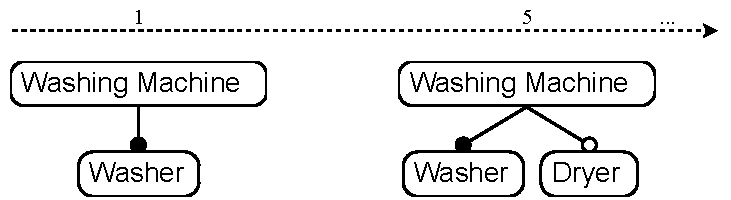
\includegraphics{WashingMachine}
  \caption{Washing machine visualisation}
  \label{ex:washing-machine-visual}
\end{figure}

\section{Operations}
\label{sec:operations}

We define \emph{update operations} to alter the interval-based feature model. The choice of operations is in large part based on the edit operations defined in our earlier work~\cite{art:consistency-preserving-evolution-planning}. We adapt them by adding a temporal dimension, letting us specify both \emph{where} an operation should be applied in the feature model, and \emph{when}, i.e. at which stage of the plan. We give a brief summary of the requirements a plan must fulfil for the operations to be applied.

\begin{itemize}
  \item \textbf{addFeature}(\var{featureID}, \var{name}, \var{featureType}, \var{parentGroupID}) from $t_n$ to $t_m$\\
      Adds feature with ID \var{featureID}, name \var{name}, and feature variation type \var{featureType} to the group with ID \var{parentGroupID} in the interval $\interval{t_n}{t_m}$. No feature with ID \var{featureID} can exist during the interval, and the name cannot belong to any other feature in the model during the interval. The parent group must exists during the interval, and the types of the feature and the parent group must be compatible, i.e., if the feature has type \mandatory{}, then the parent group must have type \andtype{}. We choose to let this operation affect the plan only within an interval so as to enable the adding of features to groups that are planned to be removed, and to add flexibility.
  \item \textbf{addGroup}(\var{groupID}, \var{groupType}, \var{parentFeatureID}) from $t_n$ to $t_m$\\
      Adds group with ID \var{groupID} and type \var{groupType} to the feature with ID \var{parentFeatureID} during the interval $\interval{t_n}{t_m}$. The group ID cannot be in use during the interval, and the parent feature must exist during the entire interval. 
  \item \textbf{removeFeature}(\var{featureID}) at time $t_n$\\
      Removes the feature with ID \var{featureID} from the feature model at $t_n$. If the plan contains a removal of the feature and a subsequent reintroduction, removing the feature at an earlier stage does not affect the reintroduction. The feature must exist at $t_n$ in the original plan for the modification to be valid. The feature must not have any child groups that are left orphaned after removal. 
  \item \textbf{removeGroup}(\var{groupID}) at time $t_n$\\
      This operation is very similar to \textbf{removeFeature}. Removes the group with ID \var{groupID} from the feature model at $t_n$, not affecting potential later reintroductions. The group must exist at $t_n$ in the original plan, and the group must not have any child features that are left orphaned after removal. 
  \item \textbf{moveFeature}(\var{featureID}, \var{targetGroupID}) at $t_n$\\
      Moves the feature with ID \var{featureID} to the group with ID $\var{targetGroupID}$ at $t_n$. The operation does not affect future moves planned for the feature. The feature's subtree is moved along with the feature. The move cannot be done if it introduces a cycle; that is, if the target group is in the feature's subtree at some point in the plan. Furthermore, the target group's type must be compatible with the feature's type, i.e. if the feature is \mandatory{} and the group is \optional{}, the move cannot be done.
  \item \textbf{moveGroup}(\var{groupID}, \var{targetFeatureID}) \\
    This operation is very similar to \textbf{moveFeature}. It moves the group with ID \var{groupID} to the feature with ID $\var{targetFeatureID}$ at $t_n$. The operation does not affect future moves planned for the group. The group's subtree is moved along with the group. If the move causes a cycle, then the modification should not be applied.
  \item \textbf{changeFeatureVariationType}(\var{featureID}, \var{newType}) \\
    Changes the feature variation type of the feature with ID \var{featureID} to \var{newType}. The change does not affect planned type changes to the feature. If the new type is \mandatory{}, the parent group type must be \andtype{}, or else the operation cannot be applied.
  \item \textbf{changeGroupVariationType}(\var{groupID}, \var{newType})\\
    Changes the group variation type of the group with ID \var{groupID} to \var{newType}. If the new type is \ortype{} or \xortype{}, and a child feature has type \mandatory{}, then the operation cannot be applied. 
  \item \textbf{changeFeatureName}(\var{featureID}, \var{name})\\
    Changes the name of the feature with ID \var{featureID} to \var{name}. It does not affect future renaming operations to the feature. No other feature may have the same name.
\end{itemize}

The operations given above cover most of the changes that are likely to be desired for a feature model evolution plan.
